\documentclass[12pt]{article}

\usepackage{enumerate}
\usepackage{amsmath}
\usepackage{amsfonts}
\usepackage{amssymb}
\usepackage{graphicx}
\usepackage{color}
\usepackage{graphics}
\usepackage{eepic}
\usepackage{wrapfig}
\usepackage[a]{esvect}

\usepackage[margin=1in]{geometry}

\usepackage{parskip}

\usepackage[theoremfont]{newpxtext}
\usepackage[varbb]{newpxmath}

\usepackage[T1]{fontenc}


\newcommand{\norm}[1]{\left\lVert {#1} \right\rVert}
\newcommand{\abs}[1]{\left\lvert {#1} \right\rvert}
\newcommand{\snorm}[1]{\lVert {#1} \rVert}
\newcommand{\sabs}[1]{\lvert {#1} \rvert}

\title{A Practical Guide to the Hessian}
\author{Ji\v{r}\'i Lebl}

\begin{document}

\maketitle

\section{Two Dimensions}

Let us start with two dimensions.
Let $f(x,y)$ be a function of two variables, and let us
find the
Taylor expansion around $(x_0,y_0)$.
Write the vector $\vec{h} = \langle x-x_0, y-y_0 \rangle$.  We
consider $\vec{h}$ as a column vector when matrices are involved.
We write $\vec{h}^t$ for the transpose, that is, the corresponding
row vector.
$$
f(x,y) = f(x_0,y_0) \, + \,
\nabla f\big|_{(x_0,y_0)} \cdot \vec{h}
\, + \,
\frac{1}{2} \vec{h}^{t} H_f\big|_{(x_0,y_0)} \vec{h} \,
+ \cdots
$$
$$
 = f(x_0,y_0) +
\underbrace{\frac{\partial f}{\partial x}\bigg|_{(x_0,y_0)} (x-x_0) +
\frac{\partial f}{\partial y}\bigg|_{(x_0,y_0)} (y-y_0)}_{\nabla
f\big|_{(x_0,y_0)} \cdot \vec{h}}
+ {}
$$
$$
{} +
\underbrace{%
\frac{1}{2} \frac{\partial^2 f}{\partial x^2}\bigg|_{(x_0,y_0)} (x-x_0)^2 +
\frac{\partial^2 f}{\partial x \partial y}\bigg|_{(x_0,y_0)} (x-x_0)(y-y_0) +
\frac{1}{2} \frac{\partial^2 f}{\partial y^2}\bigg|_{(x_0,y_0)} (y-y_0)^2}_{%
\frac{1}{2} \vec{h}^{t} H_f\big|_{(x_0,y_0)} \vec{h}}
+
\cdots
$$
The $H_f$ is the so-called \emph{Hessian matrix}
\begin{equation*}
H_f
=
\begin{bmatrix}
\frac{\partial^2 f}{\partial x^2} &
\frac{\partial^2 f}{\partial x \partial y} \\
\frac{\partial^2 f}{\partial y \partial x} &
\frac{\partial^2 f}{\partial y^2}
\end{bmatrix}
.
\end{equation*}
The quadratic form in the computation is the part
\begin{equation*}
\vec{h}^{t} H_f \big|_{(x_0,y_0)} \vec{h}
=
\begin{bmatrix}
(x-x_0) & (y-y_0)
\end{bmatrix}
\begin{bmatrix}
\frac{\partial^2 f}{\partial^2 x}\big|_{(x_0,y_0)} &
\frac{\partial^2 f}{\partial x \partial y}\big|_{(x_0,y_0)} \\
\frac{\partial^2 f}{\partial x \partial y}\big|_{(x_0,y_0)} &
\frac{\partial^2 f}{\partial^2 y}\big|_{(x_0,y_0)}
\end{bmatrix}
\begin{bmatrix}
(x-x_0) \\ (y-y_0)
\end{bmatrix}
.
\end{equation*}

\medskip

\textbf{Example:}
To see why this is so it is useful to look at a polynomial example.  The
second order approximation ought to be the best quadratic polynomial that
approximates the function.  Thus, if we look at a quadratic polynomial the
Taylor expansion up second order we should get the same polynomial, since it
itself should be its best quadratic approximation.
So consider, $f(x,y) = 1 + 2x + 3y + 4x^2+ 5xy + 6y^2$.  Compute
$$
\frac{\partial f}{\partial x} = 2 + 4 \cdot 2x + 5y, \qquad
\frac{\partial^2 f}{\partial x^2} = 4 \cdot 2, \qquad
\frac{\partial^2 f}{\partial x \partial y} = 5 ,
$$
$$
\frac{\partial f}{\partial y} = 3 + 5x + 6 \cdot 2y, \qquad
\frac{\partial^2 f}{\partial y^2} = 6 \cdot 2 .
$$
If we wish to expand this function at $(0,0)$, we compute
$$
f(0,0) = 1, \qquad
\frac{\partial f}{\partial x}\Big|_{(0,0)} = 2, \qquad
\frac{\partial^2 f}{\partial x^2}\Big|_{(0,0)} = 8, \qquad
\frac{\partial^2 f}{\partial x \partial y}\Big|_{(0,0)} = 5 ,
$$
$$
\frac{\partial f}{\partial y}\Big|_{(0,0)} = 3, \qquad
\frac{\partial^2 f}{\partial y^2}\Big|_{(0,0)} = 12 .
$$
So
\begin{equation*}
f(x,y) = 1 + 2 x + 3 y + \frac{1}{2} 8 x^2 + 5 xy + \frac{1}{2} 12 y^2 ,
\end{equation*}
and lo and behold we got the same polynomial.
Since we have the derivatives computed, we can also expand around another
point.  For example, let us expand around the point $(2,1)$
$$
f(2,1) = 40, \qquad
\frac{\partial f}{\partial x}\Big|_{(2,1)} = 23, \qquad
\frac{\partial^2 f}{\partial x^2}\Big|_{(1,1)} = 8, \qquad
\frac{\partial^2 f}{\partial x \partial y}\Big|_{(2,1)} = 5 ,
$$
$$
\frac{\partial f}{\partial y}\Big|_{(2,1)} = 25, \qquad
\frac{\partial^2 f}{\partial y^2}\Big|_{(2,1)} = 12 .
$$
So
\begin{equation*}
f(x,y) = 40 + 23(x-2) + 25 (y-1) + \frac{1}{2} 8 (x-2)^2 + 5 (x-2)(y-1) +
\frac{1}{2} 12 (y-1)^2 .
\end{equation*}

\medskip

The first order approximation gave us the gradient and thus the
steepness of the graph of $f$.  The second order approximation tells us how
the graph curves.  One particular application is in optimization, that is,
to find minima and maxima of functions, or to simply understand how a
function behaves near a critical point.

First, what is a critical point:  It is a point where the gradient is zero.
These are the candidates for maxima and minima, since at the top of the
hill, or a bottom of a valley we find that the tangent plane is horizontal,
that is, the gradient $\nabla f = \vec{0}$ is zero,
or in other words, where
$\frac{\partial f}{\partial x} = 0$ and
$\frac{\partial f}{\partial y} = 0$.

For simplicity suppose that $x_0 = y_0 = 0$, and $f(0,0) = 0$.
Further suppose that $(0,0)$ is a critical point, that is,
$\nabla f|_{(0,0)} = 0$.  Then
$$
f(x,y) = \frac{1}{2} \vec{h}^{t} H_f\big|_{(0,0)} \vec{h}
+
\cdots ,
$$
where the dots are higher order terms in the Taylor expansion.
So near the origin, $f$ behaves like a quadratic form.
Suppose that $H_f$ is nondegenerate, that is, it has
no zero eigenvalues, in other words it is invertible.

What is an \emph{eigenvalue} of a matrix $A$?
It is a value $\lambda$ for which there exists
a nonzero vector $\vec{v}$, called an \emph{eigenvector}, such that
\begin{equation*}
A \vec{v} = \lambda \vec{v} .
\end{equation*}
Recall that to compute eigenvalues you find the roots of $\det(A-\lambda I)
= 0$, which is a degree $n$ polynomial if $A$ is $n \times n$.  So finding
the eigenvalues is very hard if $n$ is large (it is very easy if $n=2$ by
using the quadratic formula).  To find an eigenvector is easy once you know
the eigenvalue: You simply find a nonzero solution to $(A-\lambda I) \vec{v}
= \vec{0}$.  That is just gaussian elimination.  Having the eigenvalues
and eigenvectors tells us everything about the matrix, but as we said
it is in general a hard problem.  Some questions (but not all)
about $A$ (and hence $H_f$) we can answer without knowing the eigenvalues.

Suppose that $\lambda$ is an eigenvalue of $H_f\big|_{(0,0)}$ and $\vec{v}$ is a
corresponding eigenvector.  As any multiple of $\vec{v}$ is also an
eigenvector, let us take $\vec{v}$ to be a unit vector,
so that $\vec{v} \cdot \vec{v} = \vec{v}^t \vec{v} = 1$.
Then parametrize the line through the origin in the direction
of $\vec{v}$.  That is,
\begin{equation*}
\vec{r}(t) = t\vec{v} .
\end{equation*}
Let us see what are the values of $f$ along the line given by
$\vec{r}(t)$.  That is we look at
\begin{equation*}
\begin{split}
f(\vec{r}(t)) & = 
f(t \vec{v}) = 
\frac{1}{2} (t \vec{v})^{t} H_f\big|_{(0,0)} (t \vec{v})
+
\cdots 
=
\frac{t^2}{2} \vec{v}^{t} H_f\big|_{(0,0)} \vec{v}
+
\cdots 
\\
& =
\frac{t^2}{2} \vec{v}^{t} \lambda \vec{v}
+
\cdots 
=
\frac{\lambda}{2} t^2 \vec{v}^{t} \vec{v}
+
\cdots 
\\
& =
\frac{\lambda}{2} t^2
+
\cdots 
\end{split}
\end{equation*}
So along the line given by $\vec{v}$, the function $f$ behaves like
the quadratic $\frac{\lambda}{2} t^2$ at least near the critical point.

If $\lambda > 0$ (that is $\frac{\lambda}{2} > 0$), then
$f(\vec{r}(t))$ has a local minimum, and if 
$\lambda < 0$, then
$f(\vec{r}(t))$ has a local maximum.  Aha!  So at least along a direction of
an eigenvector we can classify the behavior.
The Hessian is a
symmetric matrix, as
$\frac{\partial^2 f}{\partial x \partial y} = 
\frac{\partial^2 f}{\partial y \partial x}$, so $H_f^t = H_f$.  A symmetric
matrix always has real eigenvalues (no complex numbers),
and as many eigenvalues as the matrix has rows (or columns).
Futhermore, the eigenvectors of a symmetric matrix are orthogonal (at right angles): if $\vec{v}$ and
$\vec{w}$ are different eigenvectors, then
$\vec{w} \cdot \vec{v} = \vec{v}^t \vec{w} = 0$.

Suppose that $\lambda$, $\vec{v}$ is an eigenvalue / eigenvector pair,
and $\gamma$, $\vec{w}$ is another eigenvalue / eigenvector pair.  Again
taking unit eigenvectors, eigenvalues.
Writing any point $\vec{r}$ in terms of two eigenvectors
$\vec{r} = t \vec{v} + s \vec{w}$, we find
\begin{equation*}
\begin{split}
f(\vec{r}) & = 
\frac{1}{2} (t \vec{v} + s \vec{w})^{t} H_f\big|_{(0,0)} (t \vec{v} + s \vec{w})
+
\cdots 
\\
& =
\frac{t^2}{2} \vec{v}^{t} H_f\big|_{(0,0)} \vec{v}
+
\frac{s^2}{2} \vec{w}^{t} H_f\big|_{(0,0)} \vec{w}
+
\frac{ts}{2} \vec{v}^{t} H_f\big|_{(0,0)} \vec{w}
+
\frac{ts}{2} \vec{w}^{t} H_f\big|_{(0,0)} \vec{v}
+
\cdots 
\\
& =
\frac{t^2}{2} \vec{v}^{t} \lambda \vec{v}
+
\frac{s^2}{2} \vec{w}^{t} \gamma \vec{w}
+
\frac{ts}{2} \vec{v}^{t} \gamma \vec{w}
+
\frac{ts}{2} \vec{w}^{t} \lambda \vec{v}
+
\cdots 
\\
& =
\frac{\lambda}{2} t^2 \vec{v}^{t} \vec{v}
+
\frac{\gamma}{2} s^2 \vec{w}^{t} \vec{w}
+
\lambda \frac{ts}{2} \vec{v}^{t} \vec{w}
+
\gamma \frac{ts}{2} \vec{w}^{t} \vec{v}
+
\cdots 
\\
& =
\frac{\lambda}{2} t^2
+
\frac{\gamma}{2} s^2
+
\cdots 
\end{split}
\end{equation*}
For a $2 \times 2$ matrix, as in our example, the behavior
in all other directions is a combination of the two.  In terms
of $t$ and $s$, the function is $\frac{\lambda}{2} t^2 + \frac{\gamma}{2}
s^2 + \cdots$.
%The 
%There are three possible cases (if the Hessian does not have a zero
%eigenvalue).
It is really
enough to understand the matrix in the direction of the eigenvectors.

There are three possible cases in the plane as the Hessian
is $2 \times 2$:  Two positive eigenvalues,
two negative eigenvalues, or a positive and a negative.
Let us look at the representative examples.

\bigskip

\textbf{Two positive eigenvalues:}
\nopagebreak

The model case is when the matrix looks like:
\begin{equation*}
\frac{1}{2} H_f
=
\begin{bmatrix}
1 & 0 \\
0 & 1
\end{bmatrix} .
\end{equation*}
We write half the matrix for simplicity.
The function is $x^2+y^2$, and
its graph looks like:
\begin{center}
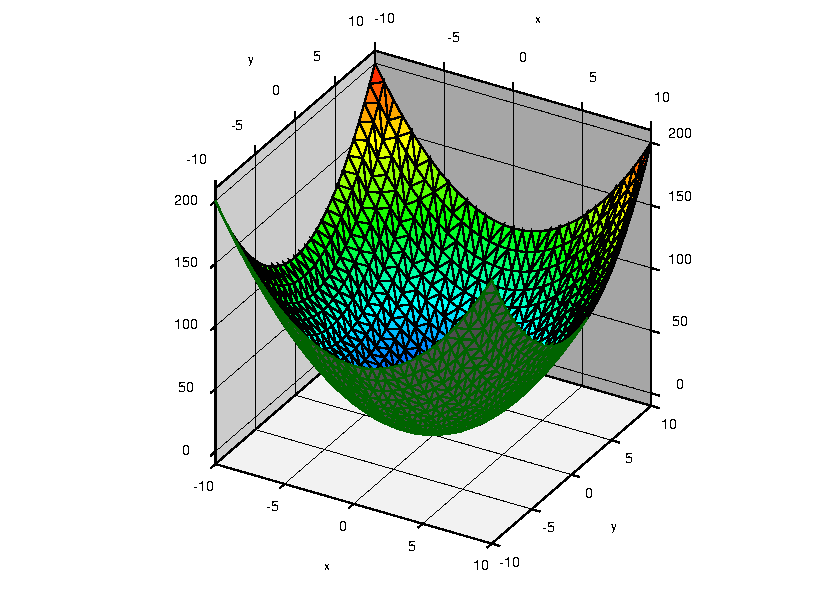
\includegraphics[width=4.0in]{xsqplusysq}
\end{center}

\bigskip

\pagebreak[2]
\textbf{Two negative eigenvalues:}

The model case is when the matrix looks like:
\begin{equation*}
\frac{1}{2} H_f
=
\begin{bmatrix}
-1 & 0 \\
0 & -1
\end{bmatrix} .
\end{equation*}
The function is $-x^2-y^2$, and
its graph looks like:
\begin{center}
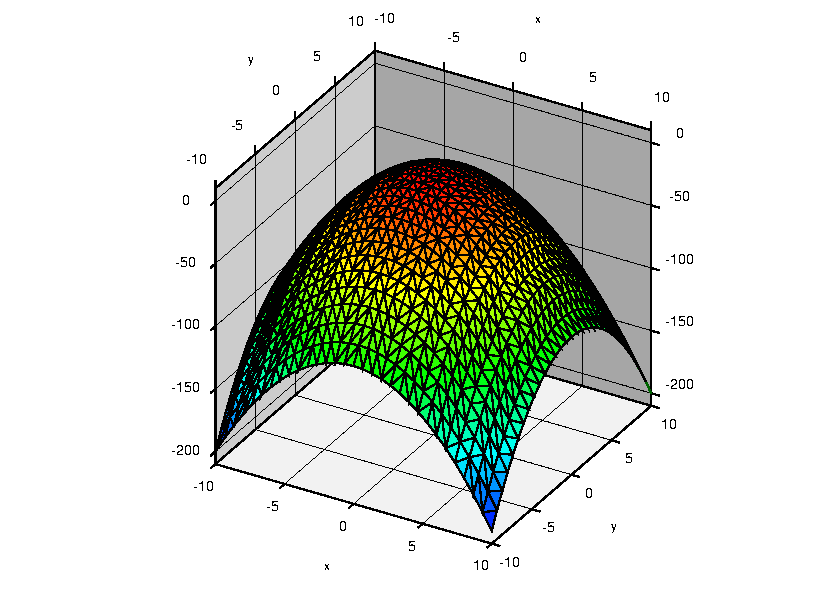
\includegraphics[width=4.0in]{minusxsqminusysq}
\end{center}

\bigskip

\pagebreak[2]
\textbf{One positive and one negative eigenvalue:}

The model case is when the matrix looks like:
\begin{equation*}
\frac{1}{2} H_f
=
\begin{bmatrix}
1 & 0 \\
0 & -1
\end{bmatrix} .
\end{equation*}
The function is $x^2-y^2$, and
its graph looks like:
\begin{center}
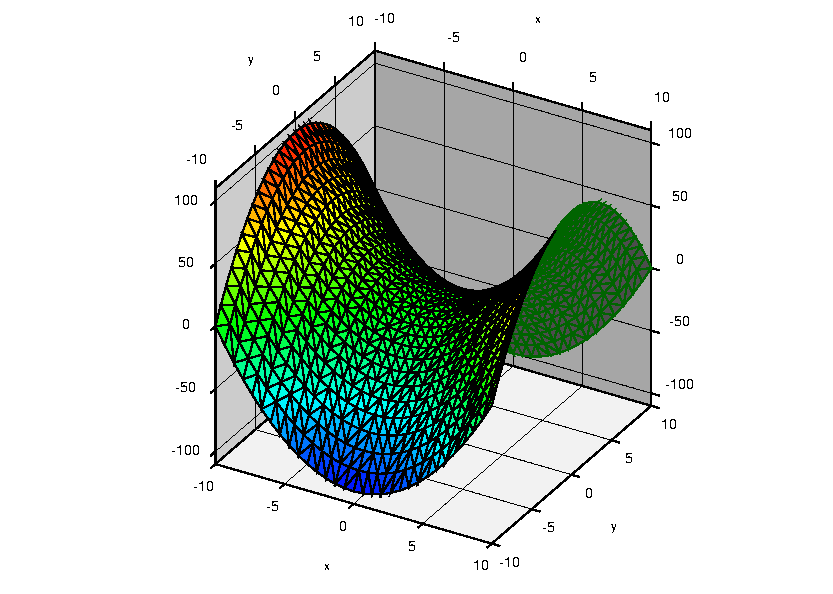
\includegraphics[width=4.0in]{xsqminusysq}
\end{center}

\bigskip

If we wish to figure out if a critical point is a minimum
or a maximum, (or a saddle), we look at the Hessian.  If it is
nondegenerate, we figure out the sign of the eigenvalues.

Computing eigenvalues is difficult, but there is a simple way to tell
the signs.  Notice
\begin{equation*}
\det\left(
\begin{bmatrix}
1 & 0 \\
0 & 1
\end{bmatrix}
\right) = 1,
\qquad
\det\left(
\begin{bmatrix}
-1 & 0 \\
0 & -1
\end{bmatrix}
\right) = 1,
\qquad
\det\left(
\begin{bmatrix}
1 & 0 \\
0 & -1
\end{bmatrix}
\right) = -1 .
\end{equation*}
The determinant of a matrix is a product of the eigenvalues.  Therefore, if
eigenvalues are of opposite signs, determinant of a $2 \times 2$ matrix is
negative.  Be careful, the reasoning is different in $3 \times 3$, or
larger, matrices.

It turns out that if you have two eigenvalues of the same sign, you can
decide on the sign of the eigenvalues of a $2 \times 2$ symmetric matrix by just
checking the upper left (or lower right) number in the matrix.  If it is
positive, then the matrix had two positive eigenvalues.  To see this,
notice that if you set $y=0$, then $f(x,0)$ is a
function of $x$ alone, and its second derivative is the upper left number of
the matrix.  If it is positive, then the graph of the function must ``curve
up'', that is, it must be a minimum.  Therefore, there must be at least one
positive eigenvalue.

\bigskip

\pagebreak[2]
\textbf{Example:}  Consider
$$
f(x,y) = 3 x^2 + 7xy  + 5y^2 .
$$
The origin is a critical point.
We just need to decide, is it a min/max or a
saddle.
The Hessian is
$$
H_f \big|_{(0,0)} =
\begin{bmatrix}
6 & 7 \\
7 & 10
\end{bmatrix}
,
\qquad
\text{and so}
\qquad
\det(H_f\big|_{(0,0)}) = 
\det \left(
\begin{bmatrix}
6 & 7 \\
7 & 10
\end{bmatrix}
\right)
=
6 \times 10 - 7 \times 7 = 11 .
$$
The product of the eigenvalues is positive, so they are of the same sign.
The critical point at the origin is either a local minimum or a maximum.
As the upper left component is 6, it must be that the surface curves
upwards, both eigenvalues are positive and the origin is a minimum for $f$.
The eigenvalues are approximately $0.72$ and $15.28$, but notice
that we didn't have to compute that.  That it is a minimum is perhaps
hard to tell from the graph.  We can mostly see the sharp sloping upwards
due to the eigenvalue $15.28$, but the sloping upwards from the center along
the ``valley floor'' due to the $0.72$ is harder to discern.
\begin{center}
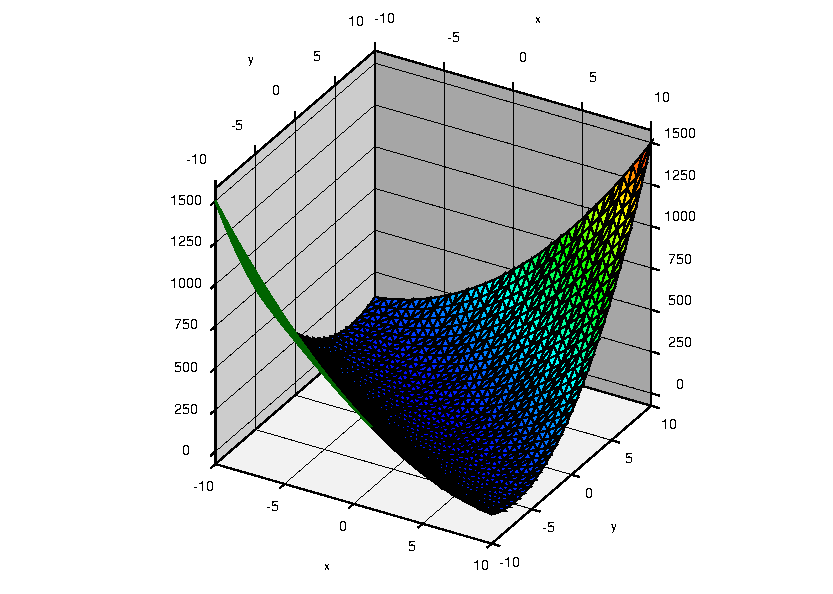
\includegraphics[width=4.0in]{all-upwards.pdf}
\end{center}

\bigskip

\textbf{Example:} Let us modify our example just a tiny bit.
Consider
$$
g(x,y) = 3 x^2 + 8xy  + 5y^2 .
$$
Again the origin is a critical point.
The Hessian is
$$
H_g\big|_{(0,0)} =
\begin{bmatrix}
6 & 8 \\
8 & 10
\end{bmatrix}
,
\qquad \text{so} \qquad
\det(H_g\big|_{(0,0)}) = 
\det \left(
\begin{bmatrix}
6 & 8 \\
8 & 10
\end{bmatrix}
\right)
=
6 \times 10 - 8 \times 8 = -4.
$$
So the eigenvalues must be of opposite signs, and the surface must be a
saddle point.  In fact, they are approximately $-0.25$ and $16.25$.
The surface turns mostly upwards, but in a certain direction, the one
corresponding to the eigenvalue $-0.25$, it turns
slightly downwards.  From drawing a graph it might not be totally easy to
immediately see that it is a saddle.  Look at how similar it is to the
previous graph.
\begin{center}
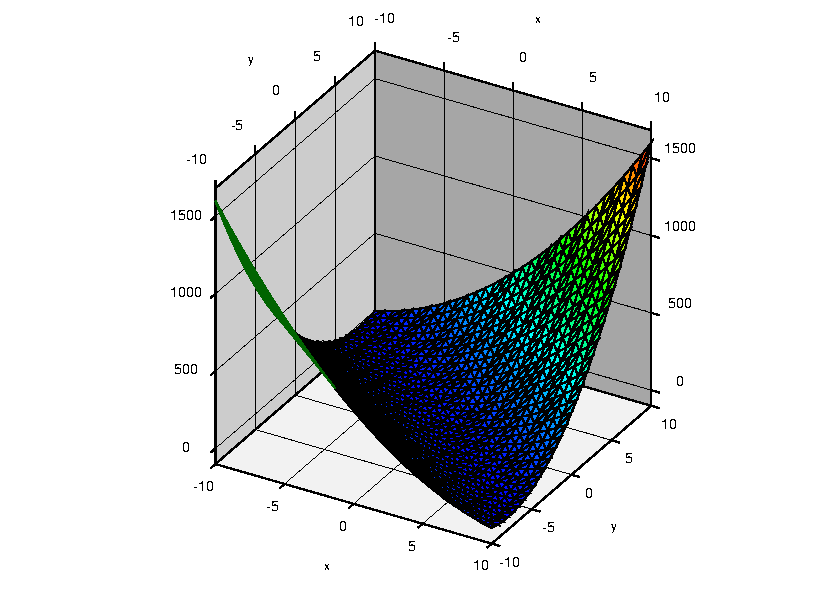
\includegraphics[width=4.0in]{mostly-upwards.pdf}
\end{center}

\bigskip

\section{Degenerate Hessian}

For a degenerate Hessian, we can sometimes read off some information, but
just not everything.  Sometimes, we do not get any information at all.

Consider
$$
f(x,y) = x^2 + y^4 .
$$
It is not difficult to convince yourself that this function is always
positive except at the origin, when it is zero.  So the origin is a minimum.
\begin{center}
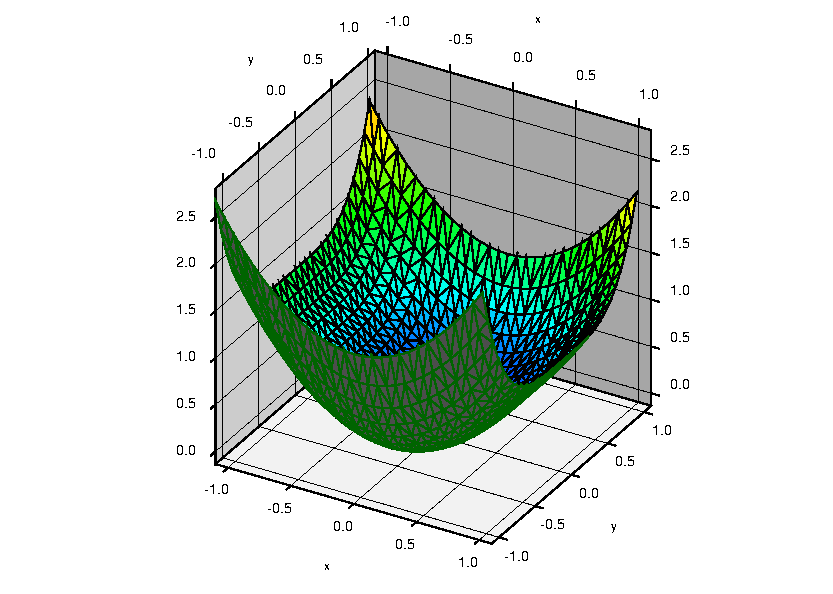
\includegraphics[width=4.0in]{degenerate-min.pdf}
\end{center}

However if you compute the Hessian  you find
$$
H_f\big|_{(0,0)} =
\begin{bmatrix}
2 & 0 \\
0 & 0
\end{bmatrix} ,
\qquad \text{so} \qquad
\det(H_f\big|_{(0,0)}) = 0 .
$$
The eigenvalues are $2$ and $0$.
The matrix is degenerate (it must have a zero eigenvalue since the
determinant is zero).  So we can't quite tell from the second derivative.

To see why we can't tell, try
$$
g(x,y) = x^2 - y^4 .
$$
The graph of this is a saddle (Just notice that $g(x,0) = x^2$ and
$g(0,y) = -y^4$).
\begin{center}
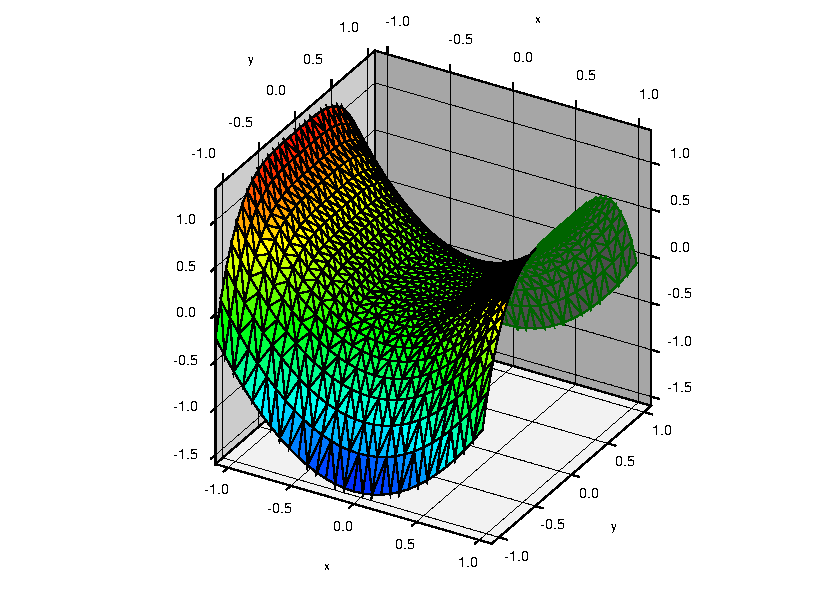
\includegraphics[width=4.0in]{degenerate-saddle.pdf}
\end{center}

Let's compute the Hessian:
$$
H_g\big|_{(0,0)} =
\begin{bmatrix}
2 & 0 \\
0 & 0
\end{bmatrix}
,
\qquad \text{so} \qquad
\det(H_g\big|_{(0,0)}) = 0 .
$$
The Hessian is the same as for $f$ above, so clearly we cannot decide
if it is a saddle or a minimum
from $H_g$ and $H_f$.  One thing that we can read off, is that the critical
point of either $g$ or $f$ is definitely not a maximum.
Along the direction of the positive eigenvalue 2, that is in the $x$
direction, we know that the function
has a minimum.  So there is no way the function has a maximum.

So if a function has a minimum, then all the eigenvalues are positive or
zero.  If the function has a maximum then all the functions are negative or
zero.  But just because a function has only positive or zero eigenvalues
does not mean the function has a minimum.

\section{Peano's example}

When the Hessian is degenerate,
one has to be careful with trying to just check for extrema (min or max) on
lines.  Consider
$$
f(x,y) = (y-x^2)(2x^2-y) .
$$
This function is zero on the sets where $y=x^2$ and $y=2x^2$, the two
parabolas in the following picture.  It is negative outside the space
between these two lines and positive between the two lines.
\begin{center}
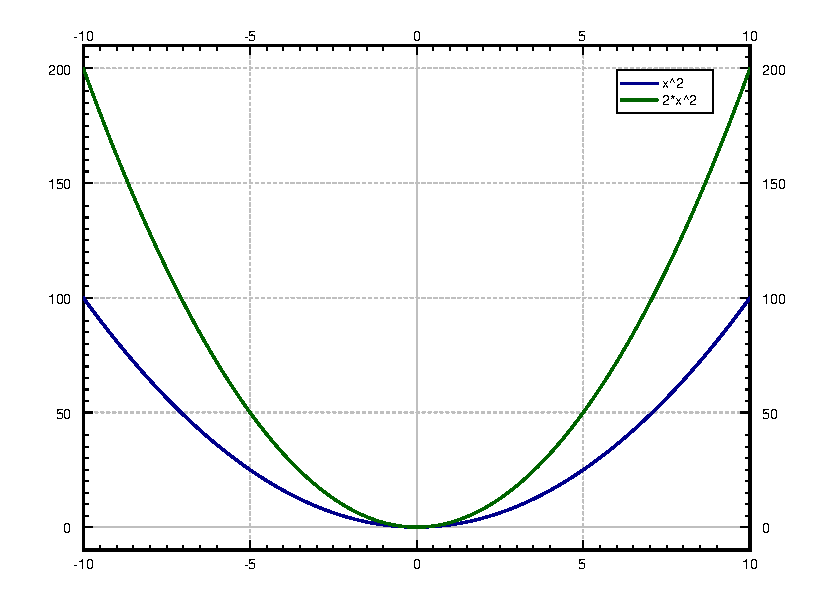
\includegraphics[width=4.0in]{peanocurves}
\end{center}
Suppose we restrict the function to any line. For example, we pick an angle
$\theta$, and consider the line through the origin at the angle 
$\theta$ to the positive $x$-axis.
This line is given by $\vec{r}(t) = \bigl\langle t \cos(\theta),t
\sin(\theta)\bigr\rangle$.  Then the restriction of $f$ to this line is
$$
f\bigl(\vec{r}(t)\bigr) = f\bigl(t\cos(\theta),t\sin (\theta)\bigr) .
$$
For any $\theta$, $f\bigl(\vec{r}(t)\bigr)$ has a strict maximum at $t=0$.
By a strict maximum we mean that the function is actually
strictly less than zero for $t$ near zero.
In fact, except for when $\theta=0$ or $\theta=\pi$, we find
$$
\frac{d^2}{dt^2} \Bigl[ f \bigl( \vec{r}(t) \bigr) \Bigr] < 0
$$
so it is a maximum (a strict one).  When $\theta = 0$ , this corresponds to
$y=0$, and so
$$
f \bigl( \vec{r}(t) \bigr) = -2t^4 ,
$$
which clearly has a strict maximum.

But $f$ is a saddle!  It is just a ``bent saddle.''
\begin{center}
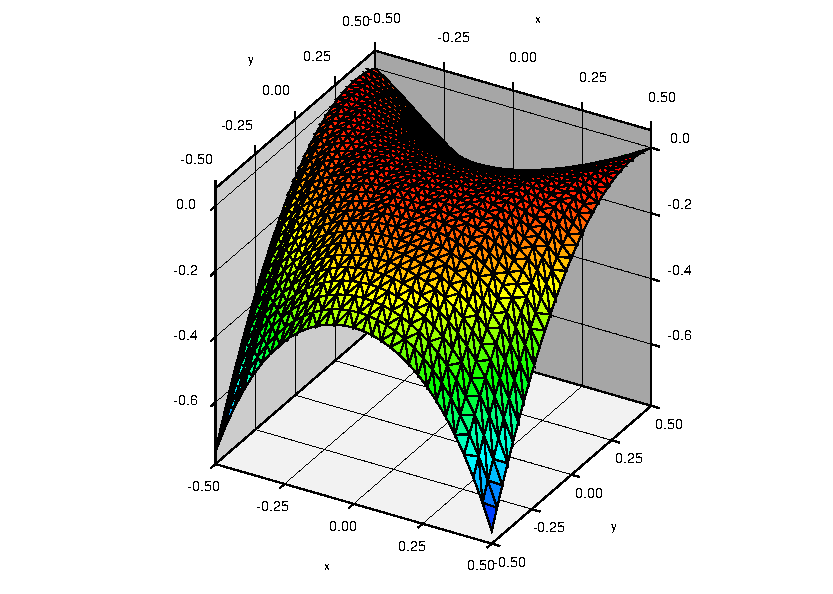
\includegraphics[width=4.0in]{peanosurface}
\end{center}
Clearly the function cannot have a min or a max since $f(0,0)=0$, but you
also have points where $f$ is positive or where $f$ is negative arbitrarily
near the origin.

A computation shows that
$$
H_f\big|_{(0,0)} =
\begin{bmatrix}
0 & 0 \\
0 & -2
\end{bmatrix}
,
\qquad \text{so} \qquad
\det(H_f) = 0 .
$$
So we wouldn't be any smarter from looking at the Hessian.

The moral of the story is that if the Hessian has zero eigenvalues, you
might have to get tricky to figure out what kind of critical point you have.
There is no simple $n$th derivative test as there is for one variable functions.

On the other hand, if the Hessian is nondegenerate, that is, it has no
zero eigenvalues, then we did answer the question by looking at lines, since
that is what looking at eigenvalues does.

\section{More Variables}

Let's consider 3 variables, with $n$ variables being exactly the same
idea.
If $f(x,y,z)$ is a function of three variables, then
the Hessian is the matrix
\begin{equation*}
H_f
=
\begin{bmatrix}
\frac{\partial^2 f}{\partial x^2} &
\frac{\partial^2 f}{\partial x \partial y} &
\frac{\partial^2 f}{\partial x \partial z}
\\
\frac{\partial^2 f}{\partial y \partial x} &
\frac{\partial^2 f}{\partial y^2} &
\frac{\partial^2 f}{\partial y \partial z}
\\
\frac{\partial^2 f}{\partial z \partial x} &
\frac{\partial^2 f}{\partial z \partial y} &
\frac{\partial^2 f}{\partial z^2}
\end{bmatrix} .
\end{equation*}

Again, a critical point is a minimum if $H_f$ has 3 positive eigenvalues, it
is a maximum if it has 3 negative eigenvalues and it is a saddle point if it
has at least one positive and one negative eigenvalue.  And if it has a
zero eigenvalue, then we can't tell how the function looks near the origin
just from looking at the Hessian.

\bigskip

\textbf{Example:}
Let
$$
f(x,y,z) = 3x^2 + xz + 2zy - z^2 .
$$
The origin is the unique critical point.
The Hessain matrix at the origin is
\begin{equation*}
H_f\big|_{(0,0,0)}
=
\begin{bmatrix}
6 & 0 & 1 \\
0 & 0 & 2 \\
1 & 2 & -2
\end{bmatrix}
\qquad
\text{so}
\qquad
\det(H_f\big|_{(0,0,0)}) = -24 < 0 .
\end{equation*}
The determinant (the product of eigenvalues)
is negative, so at least one eigenvalue is negative.  So this cannot
possibly be a minimum.  But we cannot yet decide if it is a max or a saddle.
However, we know we will be able to tell since it is nondegenerate.  We just
have to try harder.
If we would restrict to the $x$ variable, setting $y=z=0$, then we just
get the function $3x^2$, whose second derivative is $6$.  That is the $6$
in the top left corner.  Just as for the $2$ variable case, we can decide
that one of the eigenvalues must be positive since one of the diagonal
entries is positive.
Since we already know we have at least one negative eigenvalue.
The critical point must be a saddle.

Alternatively, we didn't even have to compute the determinant.  Looking at
the diagonal entries, these are always those we obtain by setting two of
the variables to zero, we have one positive, the $6$, and one negative, the
$-2$.  So we can immediately tell that the matrix has at least one positive and 
at least one negative eigenvalue.

Either running through the linear algebra or plugging into a
computer or a calculator, you find that
the eigenvalues are
approximately $-3.31, 6.13, 1.18$.  So one negative and two positive.

\bigskip

\textbf{Another example:}
Let
$$
f(x,y,z) = -9x^2 + 6xy -2y^2 -2xz -2 z^2 .
$$
The origin is a critical point.
The Hessian matrix is
\begin{equation*}
H_f\big|_{(0,0,0)}
=
\begin{bmatrix}
-18 & 6 & 0 \\
6 & -4 & -2 \\
0 & -2 & -4
\end{bmatrix}
\qquad
\text{so}
\qquad
\det(H_f\big|_{(0,0,0)}) = -72 < 0 .
\end{equation*}
Again, negative, so at least one (or possibly all three) eigenvalues are
negative.  In this case one finds that the eigenvalues are
approximately $-20.25, -0.70, -5.05$.  So all three are negative.
and the critical point is a minimum.

There is again a quick way of figuring out all three eigenvalues are
negative without computing them.  If we simply move in the $xy$ space,
setting $z=0$,
then the function should still be a minimum of two variables.  In other
words the 
the first $2 \times 2$ principal submatrix,
$\left[ \begin{smallmatrix} -18 & 6 \\ 6 & -4 \end{smallmatrix} \right]$,
should have only negative eigenvalues.  Its determinant should be positive.

OK, so we have the following test.
If the top left
entry is negative, the first $2 \times 2$ principal submatrix has positive
determinant, and the full matrix has negative determinant, then the
eigenvalues are all negative.  In this case 
\begin{equation*}
-18 < 0,
\qquad
\det \left(
\begin{bmatrix}
-18 & 6 \\
6 & -4
\end{bmatrix}
\right) = 36 > 0 ,
\qquad
\det \left(
\begin{bmatrix}
-18 & 6 & 0 \\
6 & -4 & -2 \\
0 & -2 & -4
\end{bmatrix}
\right) = -72 < 0 .
\end{equation*}
Basically you have to do some linear algebra to figure
out the signs of the eigenvalues, but you don't need to
actually compute them.

Note that it is not enough to just check the diagonal entries.  The fact
that all three are negative just says that there is at least one negative
eigenvalue.  For example, 
$$
\begin{bmatrix}
-1 & 1 & 1 \\
1 & -1 & 1 \\
1 & 1 & -1
\end{bmatrix}
$$
has eigenvalues $1,-2,-2$ (the $-2$ is repeated), so there are two negative
eigenvalues, but also a positive one, despite all diagonal entries being
negative.

So a general to figure out the signs of the eigenvalues for
a 3 by 3 (and this generalizes to $n$ by $n$) symmetric matrix is
the technique we just used above.
A symmetric matrix
\begin{equation*}
\begin{bmatrix}
a & b & c \\
b & d & e \\
c & e & f
\end{bmatrix}
\end{equation*}
has 
three positive eigenvalues if
\begin{equation*}
a > 0,
\qquad
\det \left(
\begin{bmatrix}
a & b \\
b & c
\end{bmatrix}
\right) > 0 ,
\qquad \text{and} \qquad
\det \left(
\begin{bmatrix}
a & b & c \\
b & d & e \\
c & e & f
\end{bmatrix}
\right) > 0 .
\end{equation*}
It has three negative eigenvalues if
\begin{equation*}
a < 0,
\qquad
\det \left(
\begin{bmatrix}
a & b \\
b & c
\end{bmatrix}
\right) > 0 ,
\qquad \text{and} \qquad
\det \left(
\begin{bmatrix}
a & b & c \\
b & d & e \\
c & e & f
\end{bmatrix}
\right) < 0 .
\end{equation*}
Computing determinants is a lot easier and a lot faster than computing the
actual eigenvalues.
If you do not get any zeros but the signs do not correspond to one of the
above, then you have some combination of positive and negative eigenvalues
and the critical point is a saddle.

\section{Diagonalization and change of variables}

Let us return to two variables.  Let us find the 
change of variables that makes any function into one of the three
examples.  We have almost done it before, but let's actually find
the change of variables.
So if we are allowed an (affine) linear change of coordinates, then at
a critical point, up to a constant, any
function of two variables with a nondegenerate Hessian really starts with
$f(x,y) = x^2+y^2 + \cdots$, 
$f(x,y) = x^2-y^2 + \cdots$, or
$f(x,y) = -x^2-y^2 + \cdots$.
That should surely make some computations simpler.

We have
$$
f(x,y) = f(x_0,y_0) \, + \,
\nabla f\big|_{(x_0,y_0)} \cdot \vec{h}
\, + \,
\frac{1}{2} \vec{h}^{t} H_f\big|_{(x_0,y_0)} \vec{h} \,
+ \cdots
$$

The first thing to do is to make some new coordinates where $(x_0,y_0)$ is
$(0,0)$.  So let $u = x-x_0$ and $v=y-y_0$.  As $x = u+x_0$ and $y = v+y_0$,
write
\begin{equation*}
g(u,v) = f(u+x_0,v+y_0).
\end{equation*}
The chain rule says that any derivative of $g$ is the same as the derivative
of $f$, just evaluated at the other point.  So
\begin{multline*}
\frac{\partial g}{\partial u}\Big|_{(0,0)} = 
\frac{\partial f}{\partial x}\Big|_{(x_0,y_0)}, \qquad
\frac{\partial g}{\partial v}\Big|_{(0,0)} = 
\frac{\partial f}{\partial y}\Big|_{(x_0,y_0)}, \\
\frac{\partial^2 g}{\partial u^2}\Big|_{(0,0)} = 
\frac{\partial^2 f}{\partial x^2}\Big|_{(x_0,y_0)}, \qquad
\frac{\partial^2 g}{\partial u \partial v}\Big|_{(0,0)} = 
\frac{\partial^2 f}{\partial x \partial y}\Big|_{(x_0,y_0)}, \qquad \text{etc.}
\end{multline*}

The function $g$ near the origin is expanded as
\begin{equation*}
\begin{split}
g(u,v) & = g(0,0) \, + \,
\nabla g\big|_{(0,0)} \cdot \vec{h}
\, + \,
\frac{1}{2} \vec{h}^{t} H_g\big|_{(0,0)} \vec{h} \,
+ \cdots
\\
& =
f(x_0,y_0) \, + \,
\nabla f\big|_{(x_0,y_0)} \cdot \vec{h}
\, + \,
\frac{1}{2} \vec{h}^{t} H_f\big|_{(x_0,y_0)} \vec{h} \,
+ \cdots
\end{split}
\end{equation*}
where $\vec{h} = \langle u,v \rangle = \langle x-x_0, y-y_0 \rangle$.
That is the expansion of $f(x,y)$ around $(x_0,y_0)$.

OK, we got any point to be the origin.  Let's see how we can diagonalize
$H_g$.  Given any symmetric matrix $A$ it is possible to find a matrix
$S$, such that
\begin{equation*}
A = S^t D S
\end{equation*}
where $D$ is a diagonal matrix with just $1$s, $-1$s, and $0$s on the
diagonal.  To find the matrix $S$ we take a matrix of unit eigenenvectors 
and multiply by a diagonal matrix whose entries are the square roots
of the absolute values of the eigenvalues.  Let's not worry too much about
why this $S$ works, but it is exactly what we did before, we're writing
every point as a sum of the eigenvectors, and we are also rescaling to
get rid of the sizes of the eigenvalues.

The above is the so-called \emph{Sylvester's Law of Inertia}.
The number of $1$s is the number of positive eigenvalues of $A$,
the number of $-1$s is the number of negative eigenvalues of $A$,
and
the number of $0$s is the number of zero eigenvalues of $A$.
Assuming there are no zero eigenvalues,
then for a 2 by 2 matrix, the matrix $D$ is
$\left[ \begin{smallmatrix} 1 & 0 \\ 0 & 1 \end{smallmatrix} \right]$,
$\left[ \begin{smallmatrix} -1 & 0 \\ 0 & -1 \end{smallmatrix} \right]$,
or
$\left[ \begin{smallmatrix} 1 & 0 \\ 0 & -1 \end{smallmatrix} \right]$.

So find an $S$ such that
\begin{equation*}
H_g\big|_{(0,0)} = S^t D S .
\end{equation*}
The change of coordinates is
$S \vec{h} = \vec{k}$ for some $\vec{k}$.   Then
\begin{equation*}
\vec{h}^t H_g\big|_{(0,0)} \vec{h}
=
\vec{h}^t S^t D S \vec{h}
=
(S\vec{h})^t D S \vec{h}
=
\vec{k}^t D \vec{k} .
\end{equation*}
Aha!  Let the variables be $s$ and $t$, and let
$\vec{k} = \langle s,t \rangle$ be given by
\begin{equation*}
\begin{bmatrix} s \\ t \end{bmatrix}
=
\vec{k} =
S \vec{h} 
=
S
\begin{bmatrix} u \\ v \end{bmatrix} ,
\end{equation*}
or
\begin{equation*}
\begin{bmatrix} u \\ v \end{bmatrix}
=
S^{-1}
\begin{bmatrix} s \\ t \end{bmatrix} 
=
S^{-1} \vec{k} .
\end{equation*}
Let
\begin{equation*}
\varphi(s,t) = \varphi(\vec{k}) = g(S^{-1}\vec{k}) .
\end{equation*}
The expansion of $\varphi$ around the origin
is
\begin{equation*}
\begin{split}
\varphi(s,t) & = \varphi(0,0) \, + \,
\nabla \varphi\big|_{(0,0)} \cdot \vec{k}
\, + \,
\frac{1}{2} \vec{k}^{t} H_\varphi\big|_{(0,0)} \vec{k} \,
+ \cdots
\\
& =
\varphi(s,t) = f(x_0,x_0) \, + \,
\nabla f\big|_{(x_0,x_0)} \cdot (S^{-1} \vec{k})
\, + \,
\frac{1}{2} \vec{k}^{t} D \vec{k} \,
+ \cdots
\end{split}
\end{equation*}
If $\nabla f\big|_{(x_0,y_0)} = \vec{0}$, or in other words if $\nabla
\varphi\big|_{(0,0)} = \vec{0}$, then, as $D$
is one of the three forms,
\begin{multline*}
\varphi(s,t) = f(x_0,y_0) + \frac{1}{2} ( s^2+t^2 ) + \cdots, \qquad
\varphi(s,t) = f(x_0,y_0) + \frac{1}{2} ( s^2-t^2 ) + \cdots, \\
\text{or} \qquad
\varphi(s,t) = f(x_0,y_0) + \frac{1}{2} ( -s^2-t^2 ) + \cdots
\end{multline*}
We made the Hessian be the matrix with $1$s and $-1$s on the diagonal.
If we wanted
to get rid of the $\frac{1}{2}$, we'd have to make it the matrix with $2$s
and $-2$s on the diagonal.
% That is not really crucial.
We could consider $2\varphi(s,t)$ instead.
We could also easily get rid of the constant $f(x_0,y_0)$ by just
subtracting it from $\varphi$ and consider $2(\varphi(s,t) - f(x_0,y_0))$.
Then we have $s^2+t^2 + \cdots$,
$s^2-t^2 + \cdots$, or
$-s^2-t^2 + \cdots$.

\bigskip

\textbf{Example:}
Consider
$$
f(x,y) = 3x+x^2+xy+y^2.
$$
The critical point of $f$ is where the derivative vanishes.  We leave it as
an exercise to show that there is one critical point and that is
where at $(-2,1)$.
We write $g(u,v) = f(u-2,v+1)$.  The Hessian is the matrix
\begin{equation*}
H_f\big|_{(x_0,y_0)} = H_g\big|_{(0,0)}
=
\begin{bmatrix}
2 & 1 \\
1 & 2
\end{bmatrix} .
\end{equation*}
The eigenvalues are $3$ and $1$, and the unit eigenvectors are 
\begin{equation*}
\frac{1}{\sqrt{2}}
\begin{bmatrix}
1 \\
1
\end{bmatrix} , \qquad
\frac{1}{\sqrt{2}}
\begin{bmatrix}
1 \\
-1
\end{bmatrix} .
\end{equation*}
The matrix $S$ according to the prescription above is
\begin{equation*}
S =
\begin{bmatrix}
\sqrt{3} & 0 \\
0 & 1
\end{bmatrix}
\begin{bmatrix}
\frac{1}{\sqrt{2}} &
\frac{1}{\sqrt{2}} \\
\frac{1}{\sqrt{2}} &
\frac{-1}{\sqrt{2}} 
\end{bmatrix}
=
\begin{bmatrix}
\sqrt{\frac{3}{2}} &
\sqrt{\frac{3}{2}} \\
\frac{1}{\sqrt{2}} &
\frac{-1}{\sqrt{2}} 
\end{bmatrix} .
\end{equation*}
And the matrix $D$ is just
\begin{equation*}
D =
\begin{bmatrix}
1 & 0 \\
0 & 1
\end{bmatrix} .
\end{equation*}
Then
\begin{equation*}
S^{-1} =
\begin{bmatrix}
\frac{1}{\sqrt{6}} &
\frac{1}{\sqrt{2}} \\
\frac{1}{\sqrt{6}} &
\frac{-1}{\sqrt{2}}
\end{bmatrix} .
\end{equation*}
So
\begin{equation*}
s
=\sqrt{\frac{3}{2}} u +
\sqrt{\frac{3}{2}} v 
=\sqrt{\frac{3}{2}} (x-x_0) +
\sqrt{\frac{3}{2}} (y-y_0) , \qquad
t
= \frac{1}{\sqrt{2}} u + \frac{-1}{\sqrt{2}} v 
= \frac{1}{\sqrt{2}} (x-x_0) + \frac{-1}{\sqrt{2}} (y-y_0) ,
\end{equation*}
or
\begin{equation*}
x-x_0 = x+2 = u = 
\frac{1}{\sqrt{6}} s + 
\frac{1}{\sqrt{2}} t , \qquad
y-y_0 = x-1 = v = \frac{1}{\sqrt{6}} s + 
\frac{-1}{\sqrt{2}} t .
\end{equation*}
Solve for $x$ and $y$, and plug into $f$ and check that this change
of variables really does give you
\begin{equation*}
\varphi(s,t) = -3 + \frac{1}{2} ( s^2 + t^2 ) = 3x + x^2+xy+y^2 .
\end{equation*}
The $-3$ is the $f(x_0,y_0) = f(-2,1)$.  There are no higher order terms
as $f$ had no higher order terms.

\end{document}



